\chapter{Creación de un espectáculo de \emph{video mapping}}

\section{Introducción}
En la creación de un espectáculo de \emph{video mapping} se identifican tres etapas que son el modelado de la escena, la producción del espectáculo y la proyección del mismo.

En el modelado de la escena se obtiene una representación virtual y abstracta de los objetos reales sobre los que se proyectarán. En la producción también se podrán agregar a la escena objetos no existentes en la superficie real que formarán parte del espectáculo utilizando programas computacionales para la edición del mismo.

La producción es la etapa en la que se realiza la construcción del espectáculo. Esto consiste en aplicar distintos efectos visuales sobre los objetos modelados y orquestar la ejecución de los mismos, ya sea fijando el momento en el que ocurrirán durante el transcurso del espectáculo o asociada un evento específico. Esto último podría ser por ejemplo, el presionar una tecla en la computadora.
En esta etapa también se diseña y produce la musicalización del espectáculo.

Es en la proyección del espectáculo en donde se puede contemplar el resultado de los distintos efectos visuales proyectados sobre las superficies acompañados por efectos de sonido.
Para lograr la correspondencia en la proyección de los objetos del modelo con las superficies se debe calibrar la proyección. Esta correspondencia se logra modificando el modelo de la escena, ajustando la posición y orientación de los proyectores y ajustando los parámetros intrínsecos de la proyección.

Cada una de estas etapas se puede abordar con un enfoque bidimensional o tridimensional.
Con un enfoque bidimensional, el modelo de la escena es una proyección de los objetos sobre un plano, por ejemplo una fotografía. Con un enfoque tridimensional, el modelo se mantiene independiente de un punto de vista, representándose con un conjunto de objetos tridimensionales.

%explicacion de pie de diagrama:redactarlo mejor, El modelo generado en 2d depende del punto de vista del proyector y puede no parecerse a la realidad. El modelo generado 3d se asimila a la realidad y luego con la cámara virtual ajusto el punto de vista del proyector.
\section{Enfoque 2D}
\subsection{Modelo}
Un modelo bidimensional refleja lo que vería un observador desde un punto de vista fijo.
%si se quieren agregar hay en el SVN imagenes de proyeccion perspectiva y paralela  VER
Técnicamente es el resultado de una proyección en perspectiva \cite{LibroCompGrafica} sobre un plano de vista de los elementos de la superficie a modelar.

Para la construcción se utilizan distintos orígenes como una fotografía, un plano arquitectónico de la fachada o figuras geométricas bidimensionales que representan las secciones de las superficies, en algunos casos se combinan estos métodos para obtener como resultado un único modelo.
La posición, orientación y campo de vista del proyector definirán el punto de vista y la sección de superficie que se proyectará.
\begin{figure}[H]
  \centering
    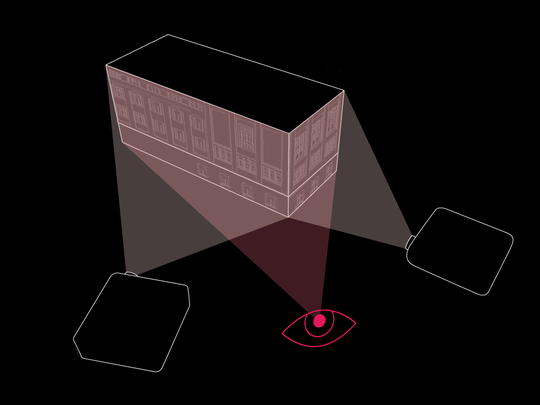
\includegraphics[width=0.7\textwidth]{./Cap2_videomapping/diagrama-2proyectores}
  \caption{Proyectores y sus puntos de vista.}
  \label{fig:diagrama-2proyectores}
\end{figure}

Cada proyector tiene un punto de vista diferente, y en caso de utilizar varios proyectores será necesario un modelo por proyector.
Algunos métodos que se utilizan para la generación del modelo son:
\begin{itemize}
  \item Una fotografía. Ubicando la cámara de forma que los puntos de vista de la cámara y del proyector coincidan minimizará los ajustes necesarios en la etapa de calibración.
  \item Un plano arquitectónico contiene información exacta de las medidas de la superficie que representa en una escala dada.Generalmente utiliza el método de proyecciones paralelas \cite{LibroCompGrafica} sobre un plano de proyección. Para utilizar el plano arquitectónico como modelo se debe transformar de forma que coincida con la proyección en perspectiva desde el punto vista que estará ubicado el proyector.
  \item Las figuras geométricas modelan sectores de la superficie donde se proyectará obviando los que no se utilizarán en el espectáculo, por esto último en comparación con los métodos anteriores logra un nivel de abstracción mayor.
Un método para generar las figuras geométricas consta en utilizar un proyector y herramientas de software que permiten delinear el contorno de las secciones de la superficie en tiempo real se observa el resultado de cada figura generada proyectada sobre la superficie validando en el momento de la construcción la correctitud del modelo. 
\begin{figure}[H]
  \centering
    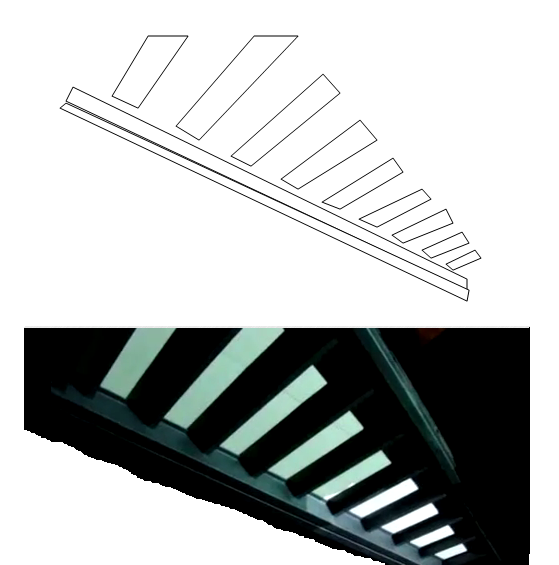
\includegraphics[width=0.7\textwidth]{./Cap2_videomapping/RepresentacionconfigurasGeometricas}
  \caption{Representación con figuras geométricas.}
  \label{fig:RepresentacionconfigurasGeometricas}
\end{figure}
Al usar el proyector para obtener el modelo queda incorporada la perspectiva del mismo y si no se modifica su posición y orientación no sería necesaria la calibración.
Otra opción es dibujar las figuras con una fotografía o plano de fondo, en este caso la construcción de las figuras geométricas se realiza delineando el contorno de la superficie en la fotografía o plano.
Una forma automática de generar el modelo es utilizando técnicas de vision por computadora\footnote{Ver glosario.} en base a algoritmos de reconocimiento de aristas \cite{ArticuloAutom2dmodel}.
\end{itemize}
\subsection{Producción del espectáculo}
La producción del espectáculo en dos dimensiones consiste en definir efectos visuales sobre regiones de un espacio bidimensional discreto\footnote{Ver glosario.} definidas en el modelo de la escena. Este espacio bidimensional discreto se representa con coordenadas de pantalla que identifican cada uno de los \emph{pixels}\footnote{Ver glosario.} del área de trabajo. Estos efectos visuales se logran realizando cualquier animación computacional que genere una salida gráfica como por ejemplo proyectando videos o imágenes sobre las regiones.
En esta etapa, además de definir los efectos se planifica en qué momento se mostrarán cada uno de ellos, pudiendo estos sincronizarse con la música que forma parte del espectáculo.

En computación gráfica se utilizan texturas para proyectar videos e imágenes sobre regiones del área de trabajo. Las texturas son mapas de \emph{bits}\footnote{Ver glosario.} utilizados para cubrir la superficie de un objeto virtual. Estos mapas de bits pueden ser generados a partir de imágenes, videos, o incluso dinámicamente mediante algoritmos computacionales permitiendo así crear efectos visuales como por ejemplo la transición de un color a otro.
Cuando se utilizan videos estos pueden ser generados teniendo en cuenta la superficie donde se está proyectando y el punto de vista desde donde se contemplará el espectáculo. Esto es particularmente importante cuando el contenido a mostrar es tridimensional, ya que para lograr una mejor ilusión, la perspectiva debe coincidir con la de los espectadores.
\begin{figure}[H]
  \centering
    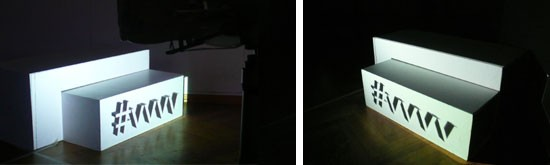
\includegraphics[width=0.7\textwidth]{./Cap2_videomapping/3dillusion}
  \caption{Ilusión 3D.}
  \label{fig:3dillusion}
\end{figure}

En este contexto se habla de mapeo, no como la salida a través de un equipo proyector, sino como la operación que logra una correspondencia entre una textura y una figura geométrica que no necesariamente coinciden en tamaño y forma. Para esto se definen coordenadas de textura en cada vértice de la figura geométrica que referencian distintas ubicaciones dentro de la misma.
Las coordenadas de las texturas tienen dos componentes, una horizontal y una vertical llamadas U y V. Si el valor de estas componentes se normaliza entre 0 y 1 entonces la esquina superior izquierda de la textura se corresponderá con la coordenada (0,0), la superior derecha con (1,0), la inferior izquierda con (0,1) y la inferior derecha con (1,1).
%agregar referencia a correspondencia de textura en un objeto, ver para imagen http://en.wikipedia.org/wiki/UV_mapping
Los vértices de una figura geométrica se asocian con coordenadas UV que definen el punto de la textura que se corresponde sobre el vértice. Mediante interpolación se logra mapear toda la textura a la figura geométrica.
Si bien es posible mapear una textura a cualquier figura geométrica, esta correspondencia es más directa utilizando un cuadrilátero ya que cada uno de los vértices se lo hace corresponder con una esquina de la textura. Es por esto que el cuadrilátero es la principal figura primitiva utilizada en las aplicaciones\footnote{Ver sección de aplicaciones relevadas.} de \emph{video mapping}.
Estos cuadriláteros se utilizan como piezas constructoras del espectáculo, cubriendo sectores del modelo sobre los cuales luego se aplican las texturas permitiendo crear los distintos efectos visuales.
\subsection{Calibración}
La calibración se utiliza para ajustar el modelo con la superficie que representa, inicialmente se fija la posición y orientación del proyector luego con ayuda de herramientas de software se aplican transformaciones geométricas al modelo para lograr la correspondencia. La transformación geométrica utilizada es una homografía\cite{LibroCompGrafica3}.
En caso de haber modificaciones en la posición y orientación del proyector la calibración deberá realizase nuevamente.

Los ajustes necesarios variarán dependiendo del método utilizado para obtener el modelo, en caso de una fotografía se obtiene desde un punto de vista fijo dado por la ubicación de la cámara, luego el proyector se ubicará de forma que el punto de vista coincida con el de la cámara, así se logra coincidencia del centro de proyección, igualmente serán necesarios ajustes ya que los lentes de la cámara y el proyector no necesariamente coincidirán en el ángulo de enfoque y distorsiones serán generadas según las propiedades del lente causando que el modelo obtenido con la cámara no se corresponda con lo que se proyectará\cite{LibroCompGrafica2}\cite{LibroPhotographicOptics}.
Con el método de generación de figuras geométricas delineando las secciones de la superficie utilizando el proyector y herramientas de software los ajustes se reducen a la posición y orientación del proyector, todas las deformaciones dadas por propiedades intrínsecas del proyector no existen.

\section{Enfoque 3D}
\subsection{Modelo}
Un modelo tridimensional a diferencia de uno bidimensional, no depende de un punto de vista sino que es una representación de cuerpos y superficies en un espacio tridimensional permitiendo al diseñador visualizar la escena desde cualquier ángulo.

Los modelos de superficie son utilizados en distintas disciplinas como la cartografía, visión computacional y gráfica computacional, su representación consta de mallas\footnote{Ver glosario.} de polígonos \cite{Mesh_building}.
Las entidades que conforman la malla son vértices, aristas, caras y atributos numéricos que representan la posición y normales de los vértices, coordenadas de textura y colores. La topología de la malla puede variar, por ejemplo los polígonos que la componen pueden tener distinta cantidad de vértices.

\begin{figure}[H]
  \centering
    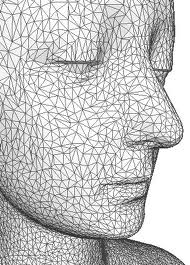
\includegraphics[width=0.7\textwidth]{./Cap2_videomapping/EjemploMallaTriangular}
    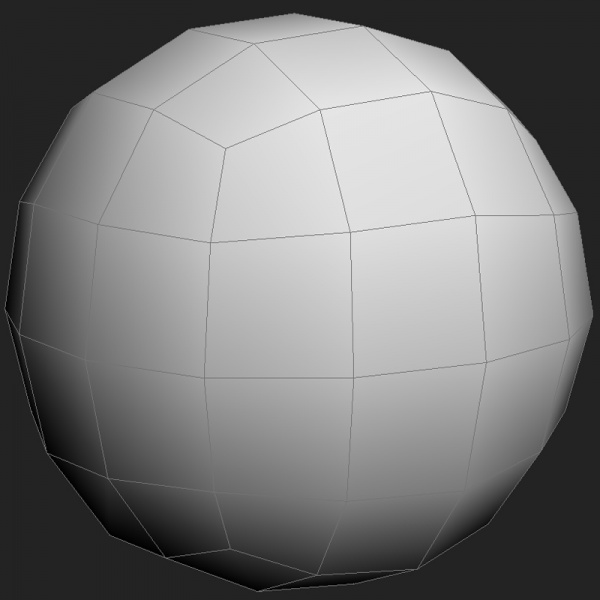
\includegraphics[width=0.7\textwidth]{./Cap2_videomapping/EjemploMalla4Vertices}
  \caption{Ejemplo de mallas triangulares y mallas de cuadriláteros.}
  \label{fig:mallas}
\end{figure}


La conectividad describe la incidencia entre los elementos, las aristas unen los vértices y juntos conforman las caras, dos caras son adyacentes cuando comparten por lo menos una arista. La valencia de un vértice es número de aristas en las que participa (que son incidentes a él) y el grado de una cara es la cantidad de aristas que la componen.
\begin{figure}[H]
  \centering
    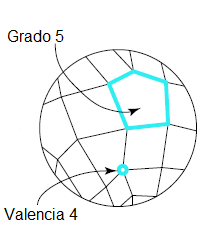
\includegraphics[width=0.7\textwidth]{./Cap2_videomapping/MallaAtributos}
  \caption{Atributos de malla.}
  \label{fig:MallaAtributos}
\end{figure}
Las mallas pueden contener información redundante, para minimizar estos casos se realizan técnicas de \emph{remeshing} que constan de algoritmos que reducen la información sin perder la representatividad de la superficie.

Existen diversas aplicaciones informáticas que permiten generar modelos tridimensionales utilizando distintas técnicas:

\begin{itemize}
  \item Poligonal modelling, a partir de mallas que representan figuras primitivas se podrán construir nuevas mallas por ejemplo aplicando operaciones de unión o resta, también se aplican transformaciones que modifican, las aristas, vértices o caras etc., aproximando el resultado a la superficie que se desea modelar.
  \item  Modelado utilizando curvas, a partir de una jaula creada por curvas se aplican transformaciones para modificarla, hundiendo o resaltando secciones aproximando el modelo a el objeto deseado, es utilizado en modelado de autos, edificios y mobiliario.
  \item Digital sculpting  es una técnica en la que software especializado provee una interfaz para modificar el modelo de forma detallada, oprimiendo y resaltando zonas de la superficie. Es utilizado para lograr efectos especiales en video juegos y películas logrando figuras y texturas subrealistas y complejas.
  \item Reconstrucción a partir de fotografías, se obtiene la representación de la superficie mediante mediciones de los objetos en las fotografías de la superficie, conociendo la escala de la imagen se extrapola y se obtiene distancia entre dos puntos en la superficie, es usada en arquitectura, ingeniería, geología, arqueología, etc.
  \item Utilizando hardware especializado, scanners 3d, se obtiene una nube de puntos que representa la superficie, generalemente la cantidad de información obtenida es densa provocando que la información capturada sea redundante, se utilizan algoritmos especializados para reducir la nube de puntos.
\end{itemize}
\subsection{Producción del espectáculo}

\subsection{Calibración}